\subsection{\newrevision{Enclosure Fabrication and Assembly Plan}}
\begingroup\color{green!45!black}
The enclosure was modeled in Fusion. A CAD interference check using simplified component envelopes found no overlap. Printing, actual board fit, clip operation, and outdoor performance require physical checks.

The proposed material is PETG. The starting Cura settings are 0.2 mm layers, four walls, 25\% body/lid infill, 100\% pad infill, a 240~$^\circ$C nozzle, and an 80~$^\circ$C bed. The body is oriented floor-down, the lid plate-down, and the pad face-down. The print plan uses two 220\,$\times$\,220 mm plates, with the body and pad on the first plate and the lid on the second. A trial print is required to check the settings, support requirements, and print time.

Assembly will fit insect mesh behind the vents, secure the boards without compressing the battery, align the USB-C opening, route OUT+ through the rib notch, and provide cable strain relief. The lid clips are then checked before strapping the box and pad separately to the trunk. Confirm the LoRa envelope, USB plug clearance, board heights, sensor-prong direction, cable diameter, foam thickness and clip force before final printing. The verified slicer output and actual purchase costs will be used to estimate material use and enclosure cost.

\begin{figure}[htbp]
\centering
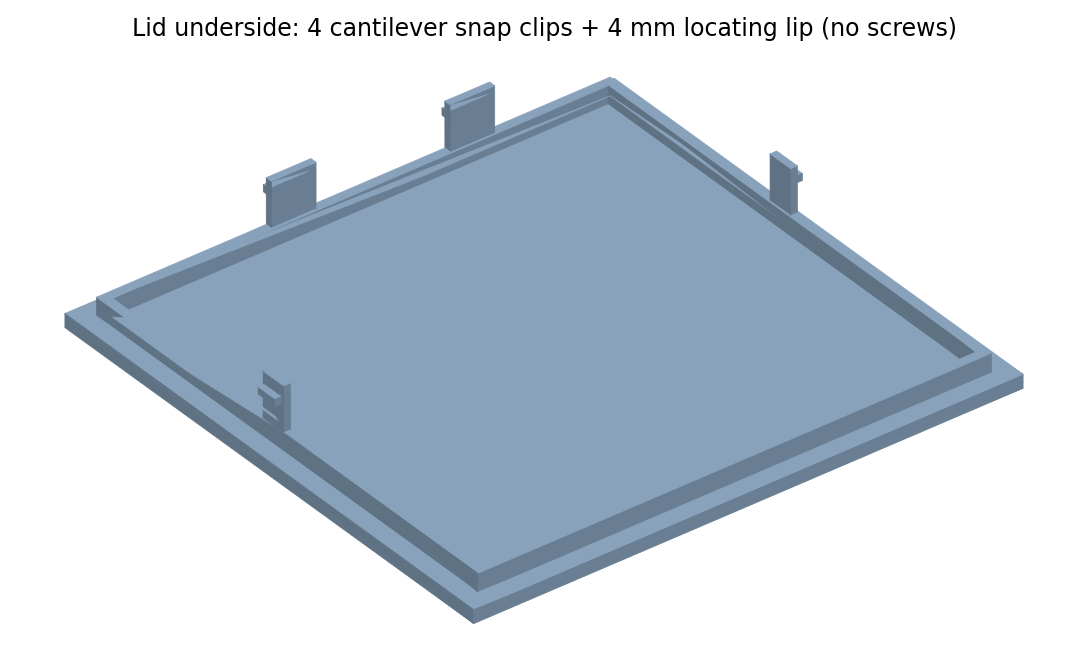
\includegraphics[width=0.49\linewidth]{figures/enclosure/04_lid_clips.png}\hfill
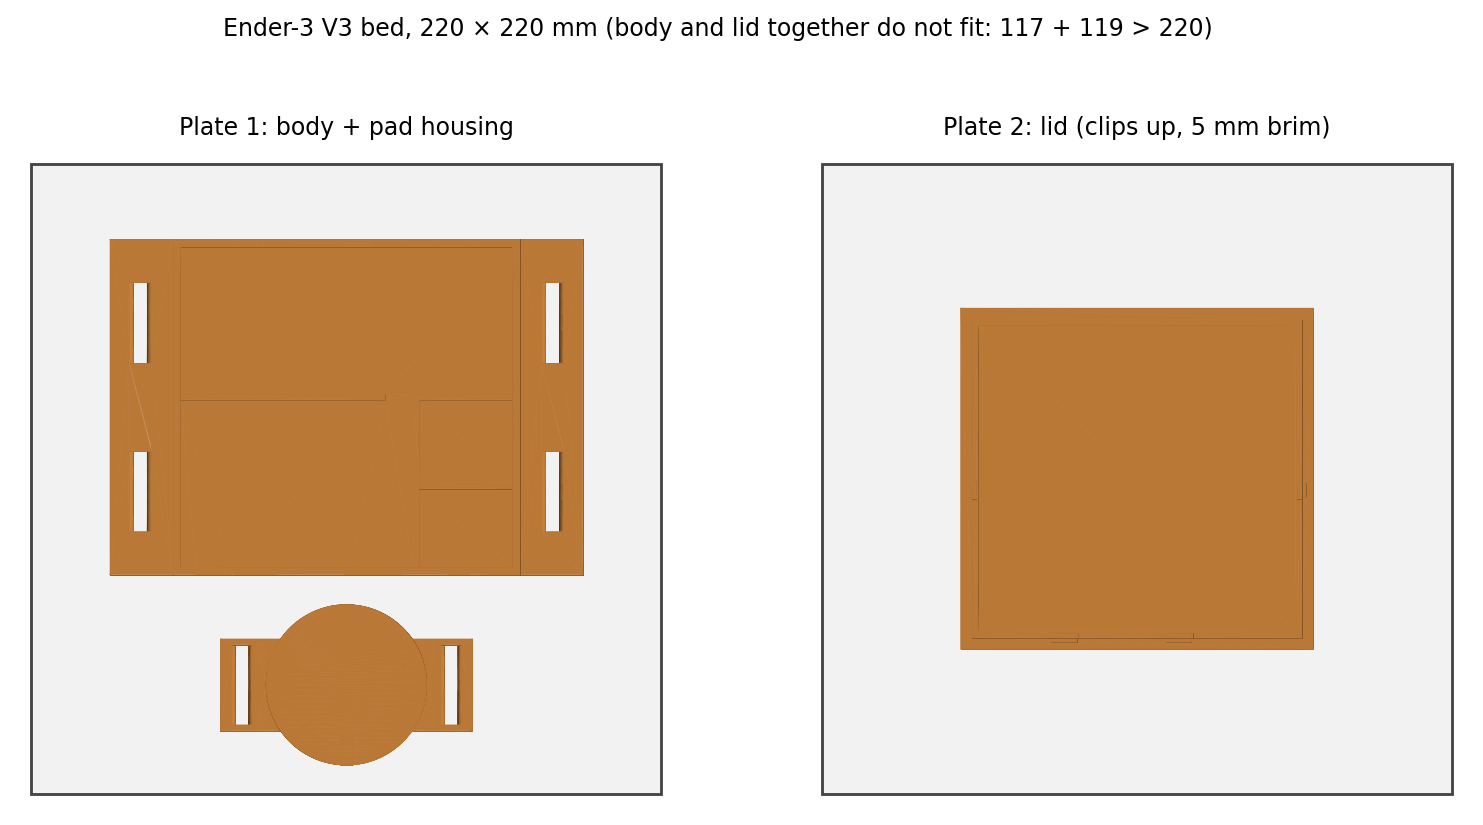
\includegraphics[width=0.49\linewidth]{figures/enclosure/06_print_plates.png}
\caption{\newrevision{CAD renders of the lid clips (left) and proposed two-plate print arrangement (right). Print orientation and fit remain to be checked in Cura and on the hardware.}}
\label{fig:enclosure_print}
\end{figure}
\FloatBarrier
\endgroup
